\section{Neural Networks}
\label{sec:neural-networks}

An artificial neural network, also referred to as ``neural network'', is a set of interconnected processing units. A processing unit receives input from external sources and connected units and computes an output which may be propagated to other units. These units represent the neurons of the human brain which are interconnected by synapses \cite[p.~23-24]{Haykin:2005}.

A processing unit consists of a propagation rule and an activation function. The propagation rule determines the actual input of the unit by mapping the output of all direct predecessors and additional external inputs onto a single input value. The activation function is then applied on the actual input and determines the output of the unit. The output of the processing unit is also called activation. This is illustrated by figure \ref{fig:processing-unit} showing a single processing unit where $f$ denotes the activation function, $z$ the actual input and $y$ the output of the unit.

\begin{SCfigure}[2\sidecaptionrelwidth][t]
	\centering
	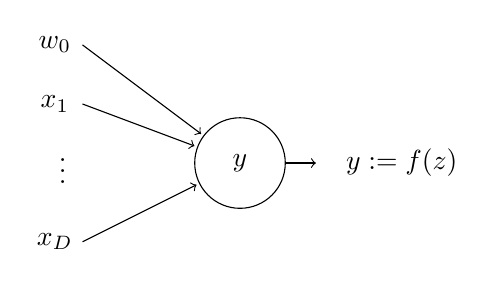
\begin{tikzpicture}[shorten >=1pt,->]
		\tikzstyle{unit}=[draw,shape=circle,minimum size=1.15cm]

		\node[unit](p) at (2,1){$y$};
		\node(dots) at (-0.25,1){\vdots};

		\draw (0,2.5) node[xshift=-10]{$w_0$} -- (p);
		\draw (0,1.75) node[xshift=-10]{$x_1$} --(p);
		\draw (0,0) node[xshift=-10]{$x_D$} -- (p);
		\draw (p) -- (3,1) node[xshift=30]{$y := f(z)$};
	\end{tikzpicture}
	\caption[Single processing units and its components.]{Single processing unit and its components. The activation function is denoted by $f$ and applied on the actual input $z$ of the unit to form its output $y = f(z)$. $x_1, \ldots, x_D$ represent input from other units within the network; $w_0$ is called bias and represents an external input to the unit. All inputs are mapped onto the actual input $z$ using the propagation rule.}
	\label{fig:processing-unit}
\end{SCfigure}

We distinguish input units and output units. Input units accept the input of the whole network and output units form the output of the network. Each input unit accepts a single input value $x$ and we set the output to $y := x$. Altogether, a neural network models a function $y(x)$ which dimensions are determined by the number of input and output units.
% For example figure \ref{fig:simple-network} shows a neural network with one input unit $p_1$ and one output unit $p_2$ such that it represents a function $y:\mathbb{R} \rightarrow \mathbb{R}$.

As to visualize neural networks we use directed graphs which we call network graphs. As illustrated in figure \ref{fig:processing-unit}, single processing units are represented by nodes and are interconnected by directed edges. The nodes of the graph are labeled according to the corresponding output.

%\begin{figure}[h]
%\begin{center}
%	\begin{tikzpicture}[shorten >=1pt]
%		\tikzstyle{unit}=[draw,shape=circle]
%
%		\node[unit](p1) at (0,0){$p_1$};
%		\node[unit](p2) at (1.5,0){$p_2$};
%
%		\draw[->] (p1) -- (p2);
%		\draw[->] (-1,0) node[xshift=-10]{$x$} -- (p1);
%		\draw[->] (p2) -- (2.5,0) node[xshift=6]{$y$};
%
%		\draw [decorate,decoration={brace,amplitude=10pt},xshift=-4pt,yshift=0pt] (-0.25,0.5) -- (2,0.5) node [black,midway,yshift=0.6cm]{neural network};
%	\end{tikzpicture}
%	\caption{Neural network with one input and one output unit.}
%	\label{fig:simple-network}
%\end{center}
%\end{figure}

\subsection{The Perceptron}
\label{subsec:perceptron}

As example we discuss Rosenblatt's perceptron which was introduced in 1958 \cite[p.~333-335]{DudaHartStork:2001}.
\begin{SCfigure}[12][b]
	\centering
    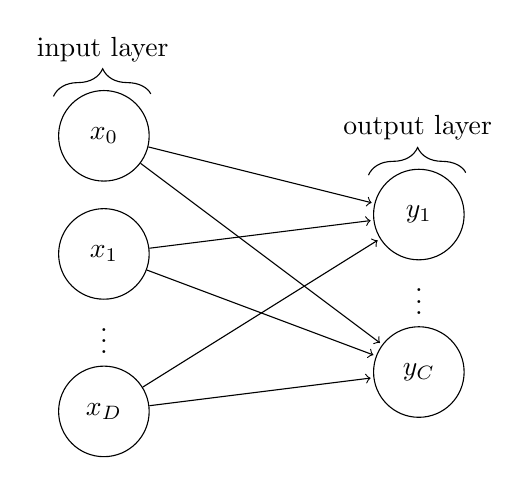
\begin{tikzpicture}[shorten >=1pt]
        \tikzstyle{unit}=[draw,shape=circle,minimum size=1.15cm]

        \node[unit](x0) at (0,3.5){$x_0$};
        \node[unit](x1) at (0,2){$x_1$};
        \node(dots) at (0,1){\vdots};
        \node[unit](xd) at (0,0){$x_D$};

        \node[unit](y1) at (4,2.5){$y_1$};
        \node(dots) at (4,1.5){\vdots};
        \node[unit](yc) at (4,0.5){$y_C$};

        \draw[->] (x0) -- (y1);
        \draw[->] (x0) -- (yc);

        \draw[->] (x1) -- (y1);
        \draw[->] (x1) -- (yc);

        \draw[->] (xd) -- (y1);
        \draw[->] (xd) -- (yc);

        \draw [decorate,decoration={brace,amplitude=10pt},xshift=-4pt,yshift=0pt] (-0.5,4) -- (0.75,4) node [black,midway,yshift=+0.6cm]{input layer};
        \draw [decorate,decoration={brace,amplitude=10pt},xshift=-4pt,yshift=0pt] (3.5,3) -- (4.75,3) node [black,midway,yshift=+0.6cm]{output layer};
    \end{tikzpicture}
    \caption[Network graph of a perceptron with $D$ input units and $C$ output units.]{The perceptron consists of $D$ input units and $C$ output units. All units are labeled according to their output: $y_i = f(z_i)$ in the case of output units; $x_i$ in the case of input units. The input values $x_i$ are propagated to each output unit using the weighted sum propagation rule. The additional input value $x_0 := 1$ is used to include the biases as weights. As suggested in section \ref{subsec:layered-networks} the units are assembled in layers.}
    \label{fig:perceptron}
\end{SCfigure}
The perceptron consists of $D$ input units and $C$ output units. Every input unit is connected to every output unit as shown in figure \ref{fig:perceptron}. For $1 \leq i \leq C$ the $i^{\text{th}}$ output unit computes the output
\begin{align}
y_i = f(z_i) \text{ with } z_i = \sum _{k=1} ^D w_{ik} x_k + w_{i0}
\end{align}
where $x_j$ is the input of the $j^{\text{th}}$ input unit. In this case the propagation rule is the weighted sum over all inputs with weights $w_{ik}$ and biases $w_{0k}$. The bias can be included as weight when considering an additional input $x_0 := 1$ such that the actual input $z_i$ can be written~as
\begin{align}
z_i = \sum _{k=0} ^d w_{ik} x_k\onedot
\end{align}

Throughout this paper we use the weighted sum as propagation rule for all units except the input units while activation functions may vary according to the discussion of the next section.

% The perceptron represents a function $y(x,w)$ where $w$ is the vector containing all variable weights. In the case of multiple input and output units we will use $y_i = y(x, w)$ to denote the output at the $i^{\text{th}}$ output unit.

\subsection{Activation Functions}

\begin{SCfigure}[\sidecaptionrelwidth][b!]
	\centering
    	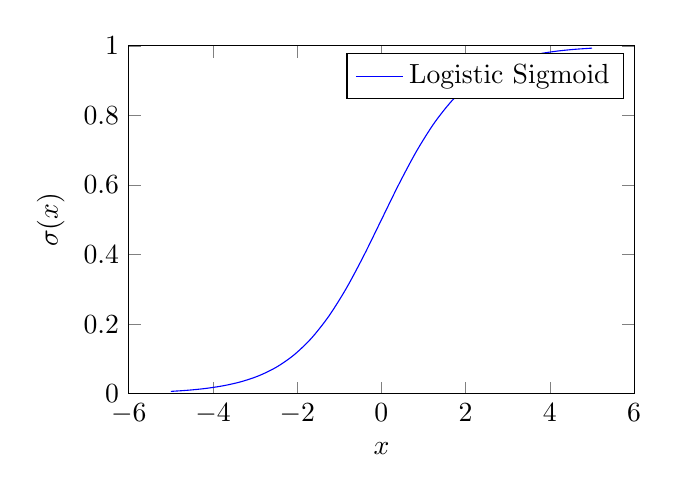
\begin{tikzpicture}
		\begin{axis}[width=8cm,height=6cm,ylabel=$\sigma(x)$,xlabel=$x$,ymin=0,ymax=1,xmin=-6,xmax=6]
			\addplot[blue,smooth] {1/(1+exp(-x))};
			\addlegendentry{Logistic Sigmoid}
		\end{axis}
	\end{tikzpicture}
    	\caption[The logistic sigmoid as activation function.]{The logistic sigmoid is a commonly used s-shaped activation function. It is both smooth and monotonic and allows an probabilistic interpretation as its range is limited to $[0,1]$.}
    	\label{fig:logistic-sigmoid}
\end{SCfigure}

The activation function determines the output of the unit. Often, a threshold function as for example the heaviside function
\begin{align}
h(z) = 
\begin{cases}
1  & \text{if } z \geq 0\\
0 & \text{if } z < 0
\end{cases}
\end{align}
is used \cite[p.~34-37]{Haykin:2005}. But in general we want the activation function to have certain properties. Network training using error backpropagation as discussed in section \ref{subsec:error-backpropagation} requires the activation function to be differentiable. In addition, we may want to use nonlinear activation functions as to increase the computational power of the network as discussed in section \ref{subsec:expressive-power} \cite[p.~307-308]{DudaHartStork:2001}.

A sigmoid function is a commonly used s-shaped function. The logistic sigmoid is given by
\begin{align}
\sigma(z) = \frac{1}{1 + \exp(-z)}
\end{align}
and shown in figure \ref{fig:logistic-sigmoid}. It can be considered as smooth version of the heaviside function. The softmax function is given by
\begin{align}
\sigma (z, i) = \frac{\exp(z_i)}{\sum _{k = 1} ^C \exp(z_k)}
\end{align}
where $C$ is the dimension of the vector $z$. Both functions are smooth and monotonic which means there are no additional local extrema. This is desirable for network training because multiple extrema within the activation function could cause additional extrema within the error surface \cite[p.~307-308]{DudaHartStork:2001}. In addition they allow a probabilistic interpretation which we use in section \ref{sec:pattern-recognition}. The derivatives of both the logistic sigmoid and the softmax function take preferable forms for implementation:
\begin{align}
\frac{\partial \sigma (z)}{\partial z} &= \sigma(z) (1 - \sigma(z))\text{,}\\
\frac{\partial \sigma (z, i)}{\partial z_j} &= \sigma(z, i) \left( \delta(i, j) - \sigma(z, j)\right)
\end{align}
where $\delta$ denotes the Kronecker delta\footnote{The Kronecker delta $\delta(i,j)$ equals $1$ if $j = i$ and is $0$ otherwise.}.

\subsection{Layered Networks}
\label{subsec:layered-networks}

Arranging the units in layers results in a layered network. Figure \ref{fig:perceptron} already introduced the perceptron as layered network. In this case we have a layer of input units and a layer of output units. We may add additional units organized in so called hidden layers. These units are called hidden units as they are not visible from the outside \cite[p.~43]{Haykin:2005}.

% Feed-forward topology can then be interpreted as follows: a unit in layer $i$ may only have an outgoing connection to a unit in layer $j$ if $j > i$. This includes connections skipping one or more layers.

For counting the number of layers we skip the input layer because there is no real processing taking place and no variable weights \cite[p.~229]{Bishop:2006}. Thus, the perceptron can be considered a single-layer perceptron without any hidden layers.

\subsection{Feed-Forward Networks}

% From the network diagram in figure \ref{fig:perceptron} we can consider a neural network as directed graph $(V,E,\omega)$ where $V$ is the set of processing units, $E$ the connections between them and $\omega: E \rightarrow \mathbb{R}$ a weight function.

Since we can model every neural network in the means of a network graph we get new neural networks by considering more complex network topologies \cite[p.229-231]{Bishop:2006}. We distinguish two network topologies:
\begin{description}
\item[Feed-forward] In a feed-forward topology we prohibit closed cycles within the network graph. This means that a unit in layer $p$ may only propagate its output to a unit in layer $l$ if $l > p$. Thus, the modeled function is deterministic.
\item[Recurrent] Recurrent networks allow closed cycles. A connection establishing a closed cycle within a network graph is called feedback connection.
%An obvious recurrent network is shown in figure \ref{fig:recurrent-network}.
\end{description}
%\begin{figure}[h]
%\begin{center}
%    \begin{tikzpicture}[shorten >=1pt]
%        \tikzstyle{unit}=[draw,shape=circle,minimum size=1.15cm]
%
%        \node[unit](x) at (0,3){$x$};
%
%        \node[unit](y) at (3,3){$y$};
%
%        \draw (x) edge[out=45,in=135,->] (y);
%        \draw (y) edge[out=215,in=325,->] (x);
%    \end{tikzpicture}
%    \caption{Simple recurrent network.}
%    \label{fig:recurrent-network}
%\end{center}
%\end{figure}
In this paper we consider feed-forward networks only. As demonstrated in figure \ref{fig:perceptron} the single-layer perceptron implements a feed-forward topology.

\subsection{Multilayer Perceptrons}
\label{subsec:multilayer-perceptron}

The multilayer perceptron has additional $L \geq 1$ hidden layers. The $l^{\text{th}}$ hidden layer consists of $m^{(l)}$ hidden units. The output value $y_{i}^{(l)}$ of the $i^{\text{th}}$ hidden unit within this layer is
\begin{align}
y_{i}^{(l)} = f\left(\sum _{k =1} ^{m^{(l-1)}} w_{ik}^{(l)} y_{k}^{(l-1)} + w_{i0}^{(l)}\right) \overset{y_{0}^{(l-1)} := 1}{=} f\left(\sum _{k = 0} ^{m^{(l-1)}} w_{ik}^{(l)} y_{k}^{(l-1)}\right)\onedot
\end{align}
Altogether, we count $(L+1)$ layers including the output layer where we set $D := m^{(0)}$ and $C := m^{(M+1)}$. Then $w_{ik}^{(l)}$ denotes the weighted connection between the $k^{\text{th}}$ unit of layer $(l-1)$ and the $i^{\text{th}}$ unit of layer $l$. Figure \ref{fig:twolayer-perceptron} shows a two-layer perceptron with $m := m^{(1)}$ units in its hidden layer. As previously mentioned, we added additional units $x_0 := y_0^{(1)} := 1$ to represent the biases.
\begin{SCfigure}[\sidecaptionrelwidth][t]
	\centering
	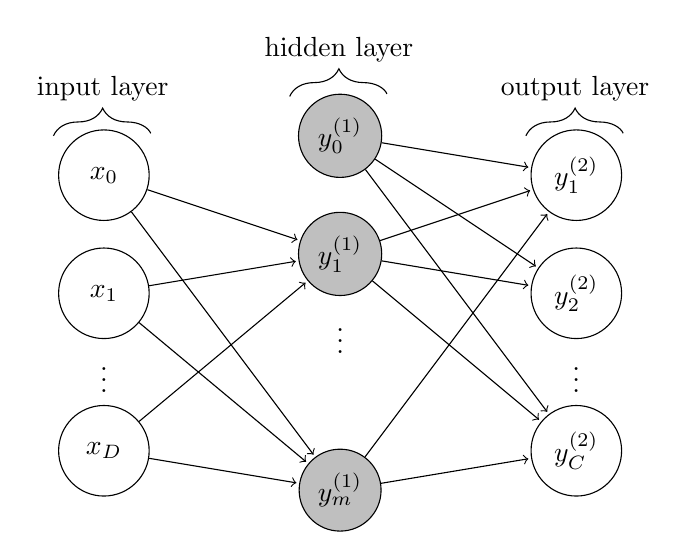
\begin{tikzpicture}[shorten >=1pt]
		\tikzstyle{unit}=[draw,shape=circle,minimum size=1.15cm]
		\tikzstyle{hidden}=[draw,shape=circle,fill=black!25]

		\node[unit](x0) at (0,3.5){$x_0$};
		\node[unit](x1) at (0,2){$x_1$};
		\node(dots) at (0,1){\vdots};
		\node[unit](xd) at (0,0){$x_D$};

		\node[hidden](h0) at (3,4){$y_0^{(1)}$};
		\node[hidden](h1) at (3,2.5){$y_1^{(1)}$};
		\node(dots) at (3,1.5){\vdots};
		\node[hidden](hm) at (3,-0.5){$y_m^{(1)}$};

		\node[unit](y1) at (6,3.5){$y_1^{(2)}$};
		\node[unit](y2) at (6,2){$y_2^{(2)}$};
		\node(dots) at (6,1){\vdots};	
		\node[unit](yc) at (6,0){$y_C^{(2)}$};

		\draw[->] (x0) -- (h1);
		\draw[->] (x0) -- (hm);

		\draw[->] (x1) -- (h1);
		\draw[->] (x1) -- (hm);

		\draw[->] (xd) -- (h1);
		\draw[->] (xd) -- (hm);

		\draw[->] (h0) -- (y1);
		\draw[->] (h0) -- (yc);
		\draw[->] (h0) -- (y2);

		\draw[->] (h1) -- (y1);
		\draw[->] (h1) -- (yc);
		\draw[->] (h1) -- (y2);

		\draw[->] (hm) -- (y1);
		\draw[->] (hm) -- (yc);

		\draw [decorate,decoration={brace,amplitude=10pt},xshift=-4pt,yshift=0pt] (-0.5,4) -- (0.75,4) node [black,midway,yshift=+0.6cm]{input layer};
		\draw [decorate,decoration={brace,amplitude=10pt},xshift=-4pt,yshift=0pt] (2.5,4.5) -- (3.75,4.5) node [black,midway,yshift=+0.6cm]{hidden layer};
		\draw [decorate,decoration={brace,amplitude=10pt},xshift=-4pt,yshift=0pt] (5.5,4) -- (6.75,4) node [black,midway,yshift=+0.6cm]{output layer};
	\end{tikzpicture}
	\caption[Network graph for a two-layer perceptron with $C$ input units, $D$ output units and $m$ hidden units.]{A two-layer perceptron with $C$ input units, $D$ output units and $m := m^{(1)}$ hidden units. Again, we introduced units $x_0 := 1$ and $y_0^{(1)} := 1$ to include the biases as weights. To distinguish units and weights with same indices in different layers, the number of the layer is written as superscript.}
	\label{fig:twolayer-perceptron}
\end{SCfigure}

In this paper we discuss the feed-forward multilayer perceptron as model for neural networks. The modeled function takes the form
\begin{align}
y(\cdot,w): \mathbb{R}^D \rightarrow \mathbb{R}^C, x \mapsto y(x,w) =
\begin{pmatrix}
y_1(x,w)\\
\vdots\\
y_C(x,w)
\end{pmatrix}
\end{align}
where $w$ is the vector comprising of all weights and $y_i(x,w) := y_i^{(L+ 1)}(x,w)$ is the output of the $i^{\text{th}}$ output unit.

\subsection{Expressive Power}
\label{subsec:expressive-power}

One of Minsky and Papert's results in 1969 showed that the single-layer perceptron has severe limitations one of which is called the Exclusive-OR (XOR) problem \cite[p.333-335]{DudaHartStork:2001}. As introduction we consider the target function $g$, which we want to model, given by
\begin{align}
g: \{0,1\}^2 \rightarrow \{0,1\}, x := (x_1, x_2) \mapsto 
\begin{cases}
1  & \text{if } x_1 = x_2 = 1\\
0 & \text{otherwise}
\end{cases}\onedot
\end{align}
Apparently, $g$ describes boolean AND. With $D = 2$ input units and $C = 1$ output unit using the $sgn(x)$ activation function, $g$ can be modeled by a single-layer perceptron:
\begin{align}
\label{eq:boolean-perceptron}
y = sgn(z) = sgn( w_{1} x_1 + w_{2} x_2 + w_{0})\onedot
\end{align}
Figure \ref{fig:boolean-perceptron} illustrates the corresponding network graph. By setting $z = 0$ we can interpret equation \eqref{eq:boolean-perceptron} as straight line in two-dimensional space:
\begin{align}
x_2 = - \frac{w_{1}}{w_{2}} x_1 - \frac{w_{0}}{w_{2}}\onedot
\end{align}
\begin{figure}[t]
\centering
\subfigure[Boolean AND (left) and boolean XOR (right) represented as classification problems.]{
    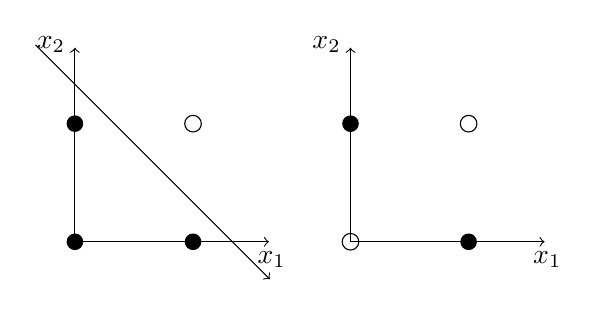
\begin{tikzpicture}[shorten >=1pt,->]
		\draw (0,0) -- (2.5,0) node[anchor=north]{$x_1$};
		\draw (0,0) -- (0,2.5) node[anchor=east]{$x_2$};
		\fill[black] (0,0) circle (3pt);
		\fill[black] (0,1.5) circle (3pt);
		\fill[black] (1.5,0) circle (3pt);
		\draw (1.5,1.5) circle (3pt);
		\draw[->] (-0.5,2.5) -- (2.5,-0.5);

		\draw (3.5,0) -- (6,0) node[anchor=north]{$x_1$};
		\draw (3.5,0) -- (3.5,2.5) node[anchor=east]{$x_2$};
		\draw (3.5,0) circle (3pt);
		\fill[black] (3.5,1.5) circle (3pt);
		\fill[black] (5,0) circle (3pt);
		\draw (5,1.5) circle (3pt);
	\end{tikzpicture}
	\label{fig:XOR}
}
\quad
\subfigure[Network graph of a single-layer perceptron modeling boolean AND.]{
    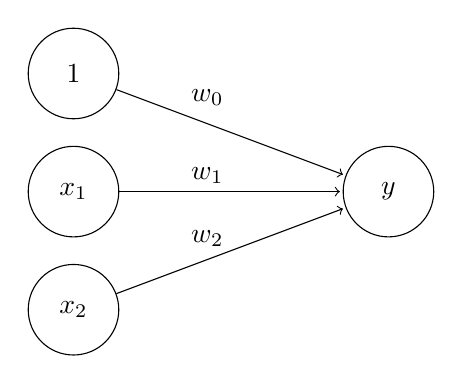
\begin{tikzpicture}[shorten >=1pt]
      		\tikzstyle{unit}=[draw,shape=circle,minimum size=1.15cm]

       	\node[unit](x0) at (0,3){$1$};
        	\node[unit](x1) at (0,1.5){$x_1$};
		\node[unit](x2) at (0,0){$x_2$};

        	\node[unit](y) at (4,1.5){$y$};

        	\draw[->] (x0) -- (y);
        	\draw[->] (x1) -- (y);
		\draw[->] (x2) -- (y);

		\node at (1.7,0.9){$w_2$};
		\node at (1.7,1.7){$w_1$};
		\node at (1.7,2.7){$w_0$};
    	\end{tikzpicture}
    	\label{fig:boolean-perceptron}
}
\caption[Single-layer perceptron for modeling boolean AND.]{Figure \ref{fig:XOR} shows both boolean AND and boolean XOR represented as classification problems. As we can see, boolean XOR is not linearly separable. A simple single-layer-perceptron capable of separating boolean AND is shown in figure \ref{fig:boolean-perceptron}.}
\label{fig:subfigureExample}
\end{figure}
A possible solution for modeling boolean AND is shown in figure \ref{fig:XOR}. But, as we can see, boolean XOR cannot be modeled by this single-layer perceptron. We say boolean XOR is not linearly separable\footnote{When considered as classification problem (see section \ref{sec:pattern-recognition}) we say the problem is not linearly separable if the classes can not be separated by a hyperplane \cite[p.~179]{Bishop:2006}.} \cite[p.~197-200]{Haykin:2005}.

This limitation can be overcome by adding at least one additional hidden layer. Theoretically, a two-layer perceptron is capable of modeling any continuous function when using appropriate nonlinear activation functions. This is a direct consequence of Kolmogorov's theorem. It states that for every continuous function $f : [0,1]^D \rightarrow \mathbb{R}$ there exist continuous functions $\psi _j : [0,1] \rightarrow \mathbb{R}$ such that $f$ can be written in the form
\begin{align}
f(x_1, \ldots, x_D) = \sum _{j = 0} ^{2D} g_f\left(\sum _{k = 1} ^D w_k \psi _j (x_k)\right)\onedot
\end{align}
But as of \cite[p.~137-140]{Bishop:1995} the function $g_f$ is dependent on $f$ and the theorem is not applicable if the functions $\psi _j$ are required to be smooth. In most applications we do not know the target function. And  the theorem says nothing about how to find the functions $\psi _j$. It simply states the existence of such functions. Thus, the theorem is not of much practical use for network design \cite[p.~287-288]{DudaHartStork:2001}. Nevertheless, the theorem is important as it states that theoretically we are able to find an optimal solution using one hidden layer. Otherwise, we could end up with a problem for which we cannot find a solution using a multilayer perceptron \cite[p.~234-235]{Haykin:2005}.